\documentclass[letterpaper,11pt]{memoir}
\usepackage[utf8]{inputenc}
\usepackage[T1]{fontenc}
\usepackage{graphicx}
\usepackage{mathpazo} % Palatino fonts for mathematics
\usepackage{tgpagella} % improved Palatino font for text
\usepackage{microtype} % better justification
\usepackage{amsmath}
\usepackage{cmap} % make PDFs searchable

% hyperref turns internal references to hyperlinks, allows \url{}
% also allows setting PDF meta information
\usepackage[pdftex,
  pdfauthor={Alex Reinhart},
  pdftitle={An Integrated System for Gamma-Ray Spectral Mapping and Anomaly
    Detection}]{hyperref} 

%% Memoir options
\chapterstyle{ell}
% Put section numbers in left margin
\setsecindent{-33pt}
% Include subsections in TOC
\setcounter{tocdepth}{3}
\setsecnumdepth{subsection}
% Caption fonts
\captionnamefont{\small\itshape}
\captiontitlefont{\small}
\captionstyle[\centering]{}

% Signature line
\newcommand{\sigline}{\noindent
\makebox[2.5in]{\hrulefill}\\}
% Date line -- shorter
\newcommand{\dateline}{\noindent
\makebox[1.5in]{\hrulefill}\\}

\begin{document}
\pagenumbering{roman}

% Title page
\begin{titlingpage}
\begin{center}
\begin{Spacing}{2}
{\LARGE
  An Integrated System for Gamma-Ray Spectral Mapping and Anomaly Detection
}
\end{Spacing}
\end{center}

\begin{center}
  Presented by Alex Reinhart\\
  Applied Research Laboratories\\
  The University of Texas at Austin
\end{center}

\begin{center}
In partial fulfillment of the requirements for graduation with the\\
Dean’s Scholars Honors Degree in Physics
\end{center}

\vskip 1in

\begin{minipage}[t]{0.5\textwidth}
\sigline 
Dr.~Alex Athey\\
Supervisor
\end{minipage}\hskip 1in
\begin{minipage}[t]{0.4\textwidth}
\dateline
Date
\end{minipage}

\vskip 0.85in

\begin{minipage}[t]{0.5\textwidth}
\sigline
Prof.~Roy Schwitters\\
Co-Supervising Professor
\end{minipage}\hskip 1in
\begin{minipage}[t]{0.4\textwidth}
\dateline
Date
\end{minipage}

\vskip 0.85in

\begin{minipage}[t]{0.5\textwidth}
\sigline
Prof.~Greg Sitz\\
Honors Adviser in Physics
\end{minipage}\hskip 1in
\begin{minipage}[t]{0.4\textwidth}
\dateline
Date
\end{minipage}
\end{titlingpage}

\cleardoublepage

\chapter*{Acknowledgments}

This work would not be possible without the support of my supervisor, Dr.~Alex
Athey, along with his colleagues at Applied Research Laboratories. Many helpful
suggestions were provided by Dr.~Steve Biegalski and Tracy Tipping of the
Nuclear Engineering Teaching Laboratories, along with experimental
support. Dr.~James Scott gave much valuable statistical advice. Bridgeport
Instruments provided helpful guidance in using their scintillator detectors. I
benefitted from the wisdom of my thesis advisor, Dr.~Roy Schwitters, and his
many suggestions. Scott Pennington lent his expertise and worked to ensure the
cooperation of UT Athletics, making our football stadium data collection
possible.

This research has been funded in part by the Office of the Deputy Assistant
Secretary of Defense for Nuclear Matters.

Finally, I must thank Rey Gomez, Patrick Vetter, Franziska Klingberg, and Todd
Hay, whose legs suffered in the name of science.

\cleardoublepage

\chapter*{Abstract}
For security, environmental, and regulatory purposes it is useful to monitor
wide areas for unexpected changes in radioactivity.  Background radiation from
naturally radioactive materials presents the largest challenge to detection
sensitivity.  Most commonly, a single background spectrum is recorded and all
subsequent spectra are compared to this static background. We have developed a
temporal anomaly detection algorithm which uses multiple passes across an area
to build a spatial map of background spectra, allowing increased sensitivity to
anomalies. By comparing spectral shape rather than count rate we increase
sensitivity and limit the influence of the background-dominated low-energy
region. To demonstrate this technique, we performed source injection
simulations, simple source detection tests, and blind tests at University of
Texas football games. Applications in wide-area monitoring through detectors on
vehicles, such as buses, are explored. We also probe the feasibility of using
kriging methods from geostatistics to provide more accurate anomaly mapping.

\cleardoublepage

\tableofcontents

\cleardoublepage

\pagenumbering{arabic}

\chapter{Introduction}

\section{Project goals}

Conducting wide-area radiation surveillance is a challenging problem for
environmental and security applications. For example, a city may wish to produce
a map of man-made gross counts over a wide region, identify
unexpected or unauthorized radioactive sources and take corrective action
\cite{Wasiolek:2007vn}. Dedicated systems have been developed, such as the
United States Department of Energy's Aerial Measuring System, which uses
aircraft to map radiological activity at nuclear sites and during emergencies
\cite{Jobst}.

It may be useful to produce regular radiation maps of an area and immediately
detect anomalies in gamma spectra, locating lost or stolen radioactive
materials, unexpected natural radioactive sources, or radiological dispersal
devices (dirty bombs). Current systems do not meet these goals: some produce
one-time static maps, rather than providing continuous monitoring, and others do
not take advantage of spatial information to more effectively detect anomalies.

We aim to construct a monitoring system which can cost-effectively map wide
areas, building maps of observed gamma spectra and rapidly detecting changes in
gamma spectra caused by new radioactive sources. To satisfy this goal, we have
constructed an integrated radiation mapping system, consisting of a mobile data
collection apparatus, spatio-temporal database of gamma spectra, and
spatially-aware anomaly mapping algorithm. We refer to this system as the
spectral comparison ratio anomaly mapping (SCRAM) system.

The SCRAM system uses mobile detectors to build spectral maps of wide-areas and
identifies temporal anomalies using spectral comparison ratios (SCRs), detecting
changes in spectral shape. By using a spatial database of observed spectra and
comparing new observations to the recorded background, a high sensitivity to
temporal anomalies is obtained.

We have tested the SCRAM system in real data collected at the Pickle Research
Campus, along with simulations of injected radioactive sources and blind tests
locating radioactive sources at large public events. The SCRAM system performs
well, locating simulated sources at long distances with small, inexpensive
detectors and detecting real medical sources in crowds at up to twenty meters.

The SCRAM system can be deployed on vehicles that naturally transit areas of
interest through their daily operations, such as patrol vehicles, municipal
buses, or unmanned aerial vehicles.  By using multiple passes of preexisting
vehicles, we expect to be able to provide high-sensitivity continuous wide-area
surveillance at minimal operational cost.

\section{Prior work}
In recent years there has been a heavy focus on radiation monitoring systems for
the detection of special nuclear material (SNM), usually at ports and border
crossings.\cite{Runkle:2005,Boardman:2012ca} These systems are usually portal
monitors: cargo, such as trucks or cargo containers, travels through detectors
as part of the customs process, and suspicious cargo is flagged for further
inspection. Improved techniques to distinguish between SNM and benign
radioactive sources are being developed, and portal monitors are routinely
deployed at American borders.

Techniques for monitoring wide areas have been explored less. General Electric's
Research Center has developed a Standoff Radiation Imaging System which uses a
large array of gamma detectors to provide gamma imaging at distances up to 100
meters; however, this requires a large and heavy apparatus with nearly 400
photomultiplier tubes and two dozen sodium iodide scintillators contained in a
commercial cargo van.\cite{Zelakiewicz:2011ig} 

More practical approaches have been tested by Pacific Northwest National Labs,
using commercial scintillators in a van which report an anomaly whenever the
spectral shape changes too rapidly.\cite{Pfund:2007,Pfund:2010hm} The
slowly-changing natural background is tracked with Kalman filters or an
exponentially-weighted moving average. This method is flexible enough to allow
for the automated rejection of nuisance sources (such as medical isotopes), but
performs no mapping and has no spatial awareness: the proposed algorithm simply
compares newly observed spectra to recently observed spectra, without
considering the motion or location of the vehicle. This makes the algorithm
oblivious to small or distant sources, which are easily confused with slow
changes in the natural background spectrum.

Current mapping techniques, however, are impractical. The most common method
uses helicopter- or aircraft-mounted gamma scintillators flown in a regular
pattern over a target area, at considerable expense.\cite{Wasiolek:2007vn}
Mapping of a large city may take days or weeks, rendering routine anomaly
detection expensive and impractical. We would like to combine a practical
mapping technique with previously developed spectral anomaly detection methods
to produce a more sensitive and useful system.

\section{Scope}

In this thesis, I describe four steps on the path to a practical wide-area
radiation surveillance system:

\begin{enumerate}
  \item Construction of a mobile spectral data collection system.
  \item Development of a spectral anomaly detection system.
  \item Development of a simulation system capable of simulating multiple
    radioactive sources and varying natural background radiation.
  \item Evaluation and testing of the system with data collection at the Pickle
    Research Campus and public events.
\end{enumerate}

Some work remains to produce a truly practical field-ready system, such as the
development of battery-powered lightweight mobile data collection units,
wireless data transmission and collection, and real-time analysis and
mapping. Applied Research Laboratories intends to pursue these goals in future
work. 

In Chapter~\ref{kriging}, I discuss a possible alternative algorithm to the one
discussed and developed in this thesis. The alternative method, making use of
geostatistical models such as kriging, has promise for more practical and useful
anomaly mapping systems, but has not yet been fully developed. I have developed
a pilot system and performed preliminary simulation studies to characterize its
behavior.


\chapter{Methods}

\section{Data acquisition and mapping}

We have constructed an spectral integrated data acquisition and mapping system,
consisting of a Bridgeport Instruments cesium iodide scintillator detector, GPS
interface, and Windows laptop. Spectral data is recorded into a
PostGIS\cite{postgis} database on the laptop, along with each observation's GPS
location and timestamp.

\subsection{Scintillator interface}

The Bridgeport Instruments scintillator connects to the laptop via a simple USB
interface, with drivers provided by Bridgeport. A simple C API is provided with
documentation, allowing users to control the scintillator's high voltage power
supply, photomultiplier tube settings, and integrated multichannel
analyzer. Because our data analysis code was written in Python, it was necessary
to write a Python C extension which allows Python code to interface with the
detector.

The resulting \texttt{emorpho\_cpython} module is available at
\url{https://github.com/capnrefsmmat/emorpho-cpython}. It allows Python code to
connect to a scintillator detector over USB, alter its voltage and gain
settings, and collect either histograms or raw lists of counts. Statistics, such
as detector temperature, runtime and count rates, can be read off of the
device. The result is much easier to use than the raw C interface. The module is
compatible with Python 2.7.

\subsection{Recording of spectra}

The recording, analysis and mapping code is available online at
\url{https://github.com/capnrefsmmat/radmonitor}. Spectra were recorded at
two-second intervals by the monitoring code, along with the most recent
latitude, longitude and altitude provided by the GPS unit. These data were saved
in the PostGIS database along with detector temperature, estimated GPS
horizontal dilution of precision, current time, and gamma count rate.

Occasionally the GPS signal would be lost due to overhead obstructions. In these
cases, the system continues to record spectra, but without an attached location;
it is hoped that future work will allow these locations to be interpolated from
those recorded just prior to signal loss.

The monitoring system also runs a local webserver. Browsers viewing
\texttt{http://localhost:8080} are presented with a real-time graph of current
count rates and GPS precision, along with detector temperature and other
diagnostic data. This display was made available over a WiFi connection so the
detector could be monitored in real-time via smartphone, and was successfully
used to collect several hours of data.

\subsection{Mapping}

We used the \texttt{matplotlib}\cite{Hunter:2007} library for Python, along with
the Basemap Toolkit, to perform graphical mapping. During analysis, GPS latitude
and longitude coordinates were converted by PostGIS to the NAD83 (NSRS2007)
Texas Central (SRID 3663) coordinate system, a Lambert Conic Conformal
projection suitable for use in central Texas.\cite{nad83} All units are in
meters. This was substantially easier than working in latitude and longitude,
allowing observations to be placed on a Euclidean plane rather than a spheroid.

For reference, maps were plotted on top of OpenStreetMaps data of the local
area, including local building outlines and streets.\cite{osm} Observed count
rates were plotted as hexagonally-binned chloropleth maps. Spectral analysis was
done on square spatial bins, with each bin plotted with a color indicating the
spectra difference observed.

\section{Spectral comparison ratio anomaly detection}

The final component of the SCRAM system is our spectral anomaly detection
algorithm. This does not detect changes in radiation levels, but instead
examines spectral shapes. SCR collects observed gamma counts into energy bins,
which may be chosen to cover certain spectral regions of interest or can be
distributed evenly across the spectrum. Various methods exist to choose energy
bins targeted for detection of particular
isotopes;\cite{Wei:2010go,Pfund:2010hm} however, for this demonstration, we
simply chose 8 energy bins which contained roughly equal numbers of counts in a
typical background spectrum, covering the energy range between 100 and 2500 keV.

Binning the data into \(n\)
bins creates a vector of counts \(\mathbf{c} = [ c_1 c_2 \ldots c_n]\). We also
have a background vector, \(\mathbf{b}\), containing the mean observed spectrum
across all background observations, binned in the same way.  One energy bin is
chosen as the reference bin (in this case, bin 1). The choice of reference bin
is unimportant, as the anomaly statistic is invariant to the choice of bin
\cite{Runkle:2009ev}. The spectral comparison ratios can then be computed by:
\begin{equation}\label{scr}
s_i = c_1 - \frac{b_1}{b_i} c_i,
\end{equation}
for \(i > 1\). This is mathematically equivalent to multiplying the vector
\(\mathbf{c}\) by a spectral shape matrix \(S\):

\begin{equation}
S = \begin{pmatrix}
1 & - \frac{b_1}{b_2} & 0 & \ldots & 0 \\
1 & 0 & - \frac{b_1}{b_3} & \ldots & 0\\
\vdots \\
1 & 0 & 0 & \ldots & -\frac{b_1}{b_n} \\
\end{pmatrix}
\end{equation}

\begin{equation}
\mathbf{s} = S \cdot \mathbf{c}
\end{equation}

There are \((n - 1)\) linearly independent SCRs, since one bin is a reference
bin.  The SCR process compares \(c_1\) against projections based on the ratio
between bins in the background data and the counts in bin \(i\); the deviations
of the projections are given in the SCR vector \(\mathbf{s}\).  Since
\(\mathbf{s}\) is computed using ratios between bins, it is insensitive to
global changes in count rate unless they alter the spectral shape.  This
important feature allows for comparisons of spectra made with unequal
observation times.

With these useful properties, the SCR vector can be used to detect
\textit{spectral anomalies} based upon sound statistics, assuming an underlying
Poisson distribution.  Additionally, the statistical formulation allows for a
quantitative comparison between an observation's spectrum and previously
recorded observations.

\subsection{Characterizing expected variation}

To accurately detect anomalies, we first need to determine what variation can be
expected in the natural background. First, we assume that counts in each energy
bin are roughly Poisson-distributed. This would imply that the variance of the
count rate in a region is equal to its mean, which is not true in larger spatial
regions, as count rates become overdispersed. (See
Fig.~\ref{poisson-dispersion}). Consequently, we approximate that \(\text{var}
(c_i) = V c_i\), where \(V\) is the average variance-to-mean ratio of count
rates (\(V=1\) for perfectly Poisson-distributed counts). We know the
relationship between the variance of random variables:
\begin{equation}
\text{var}(aX + bY) =
a^2 \text{var}(X)  + b^2 \text{var}(Y) +  2 ab\, \text{cov}(X,Y)
\end{equation}

Hence, using (\ref{scr}) we may estimate \(\text{var}(s_i)\):

\begin{equation}
  \text{var}(s_i) = V c_1 + \left(\frac{b_1}{b_i}\right)^2 V c_i - 2
  \frac{b_1}{b_i} \text{cov}(c_1, c_i)
\end{equation}

The covariance \(\text{cov}(c_1, c_i)\) would ideally be estimated from all
previous background observations made in a spatial bin, so that
\(\text{cov}(c_1, c_i) \propto \text{cov}(b_1, b_i)\). However, spatial mapping
would be impractical if it required numerous repeated observations before
detecting anomalies. The relationship between the covariance \(\text{cov}(b_i,
b_j)\) and the correlation \(\text{corr}(b_i, b_j)\) is \cite{Morrison}:

\begin{equation}
  \text{cov}(b_i, b_j) = \text{corr}(b_i, b_j) \sqrt{\text{var}(b_i) \, \text{var}(b_j)}.
\end{equation}

To replace \(\text{cov}(c_1, c_i)\) with this we must also rescale;
\(\mathbf{b}\) may have resulted from an observation of a different length than
\(\mathbf{c}\). Consequently, we can replace the covariance with a correlation:
\begin{equation}\label{vars}
  \text{var}(s_i) = 
  V\left(c_1 + \left(\frac{b_1}{b_i}\right)^2 c_i - 2 \frac{b_1}{b_i}
  \left(\frac{T_c}{T_b}\right)^2 \text{corr}(b_1, b_i) \sqrt{b_1 b_i}\right),
\end{equation}
where \(T_c\) is the time taken to observe \(\mathbf{c}\) and \(T_b\) the time
taken to observe \(\mathbf{b}\). This is obtained by replacing
\(\text{var}(b_i)\) with \(\text{var}(b_i T_c/T_b)\), and likewise for \(\text{var}(b_j)\).

To compute \(\text{corr}(b_1,b_i)\) we do not rely only on background
observations made in the chosen spatial bin, as there is frequently not enough
data to make this possible. Instead, \(\text{corr}(b_1,b_i)\) is estimated from
observations in all bins by summing together observations into thirty-second
intervals. The correlation between bins in these summed observations is easily
computed.

Finally, we can compute the covariance matrix \(\Sigma\) between bins in the SCR
vector:
\begin{equation}
\Sigma_{ij} = \text{corr} (s_i, s_j) \sqrt{\text{var}(s_i) \text{var}(s_j)},
\end{equation}
where \(\text{corr} (s_i, s_j)\) is estimated by summing all observations across
all spatial bins in the same way as for \(\text{corr}(b_i,b_1)\), then comparing
each observation to the global mean spectrum to produce \(\mathbf{s}\).

% This following paragraph should be more convincing. -- 
% no kidding.

By using correlation matrices we have produced an anomaly detection method that
performs well with few past observations. Because the correlation matrices are
produced using all background observations, rather than only observations made
in a particular spatial region, there are sufficient observations for
well-conditioned and invertible matrices. A simpler method may be to directly
compute the covariance matrix in a single spatial bin, but this is only
practical if there are numerous observations, requiring repeated mapping passes;
covariance matrices are frequently singular or ill-conditioned
otherwise. Approaches based on shrinkage estimators are possible
\cite{Daniels:2001et}, but cannot work if there are only one or two
observations.

The correlation matrices may be computed and reused for anomaly detection in all
spatial bins; any similar method using covariance matrices would require each
spatial bin to contain observations of equal length each day, or require new
covariance matrices to be computed for each spatial bin. 

This method does rest on several assumptions; namely, gamma-ray counts must be
roughly Poisson-distributed, and the typical spectral variance should be roughly
the same over the entire region. When these assumptions are violated, the
resulting covariance matrices are likely too inaccurate to be of value.

\subsection{Anomaly detection}

Previous work has developed a simple anomaly detection algorithm which makes use
of the SCR vector \(\mathbf{s}\) \cite{Pfund:2007}. In these applications a set
of many independent background observations \(\mathbf{b}\) are made, and
\(\mathbf{s}\) is calculated for each observation. After computing the
covariance matrix \(\Sigma\) for the resulting set of SCR vectors,
\(\mathbf{s}\) is calculated for the new observation and it is compared to the
background through the Mahalanobis distance:

\begin{equation}
\label{dist}
D^2 = \mathbf{s}^T \Sigma^{-1} \mathbf{s}
\end{equation}

The Mahalanobis distance estimates the distance between a multivariate
observation and the typical mean \cite{Morrison}.  If the estimated covariance
matrix \(\Sigma\) is accurate and the background radiation source is unchanging,
the Mahalanobis distance \(D^2\) should be \(\chi^2\)-distributed with \((n-1\))
degrees of freedom. In practice there are slight background fluctuations from
various natural processes, and the distribution departs slightly from
theoretical predictions \cite{Pfund:2010hm}.

By setting a desired alarm threshold \(D_A\) based on typical natural spectral
variations, one can search for unusually large spectral anomalies, which may
indicate source changes. To monitor a wide area, observations can be aggregated
into spatial bins and the cumulative spectrum in each bin compared to previous
observations. Each bin may contain different numbers of observations, and an
individual bin may have observations at different times and locations from day
to day.

The method does not distinguish between
equally-sized anomalies from natural or artificial sources, though the choice of
energy bins may be made to optimize sensitivity to certain
isotopes \cite{Pfund:2007}. Additional benefits of this approach include being
able to detect unexpected decreases in radioactivity as well as source
substitution, which may maintain a constant count rate in a given area while
altering the spectral shape.

\section{Radioactive source simulation}
\label{simulation}
A useful tool in the evaluation of the SCRAM system is simulation. We have
constructed a full-featured radiation simulation system, allowing the simulated
injection of radioactive sources in varying background radiation fields.

The simulation system starts with a set of preexisting observations. The user
may specify the location and size of new radioactive sources to inject into
current observations. For each observation, the distance \(r\) between the
observation and each source was computed; the effective count rate \(c\) at this
distance was computed as

\begin{equation}\label{attenuation}
c(r) = \frac{Cs}{S}  \frac{R^2}{r^2} e^{-\mu (r+R)},
\end{equation}
where \(\mu\) is the effective attenuation of gamma rays in air (\(1.0003 \times
10^{-2} \text{ m}^{-1}\) for 660 keV gamma rays), \(s\) the activity of the
source, and \(S\), \(C\), and \(R\) calibrations from a known source. For
example, with our detector we found that at \(R=5\text{ cm}\), a cesium-137
source with activity \(S=8.44 \times 10^{-4} \text{ mCi}\) causes \(C=630 \text{
  counts/s}\) above background.

This result was derived from the known exponential and geometric attenuation of
gamma rays over a distance,

\begin{equation}
c(r) \propto \frac{e^{-\mu r}}{r^2}
\end{equation}
One can then take the ratio between \(c(r)\), which is unknown, and \(c(R)\),
which was observed experimentally, deriving Eq.~\ref{attenuation}.

Once the effective count rates from all simulated radioactive sources were
computed, sample spectra from each source were scaled to match the calculated
count rate and added to the observed spectrum. The new spectrum was saved to the
database as a new observation at a user-specified time, and the process repeated
for all observations in the chosen simulation window.

The result of an example simulation is shown in
Fig.~\ref{scr-injected-prc}. More complex simulations are possible; for
instance, the system may also simulate a constant background spectrum at a
user-chosen count rate, along with multiple independent radioactive point
sources with separate spectra. Multiple repeat observation passes can be
created.

\begin{figure}
  \centering
  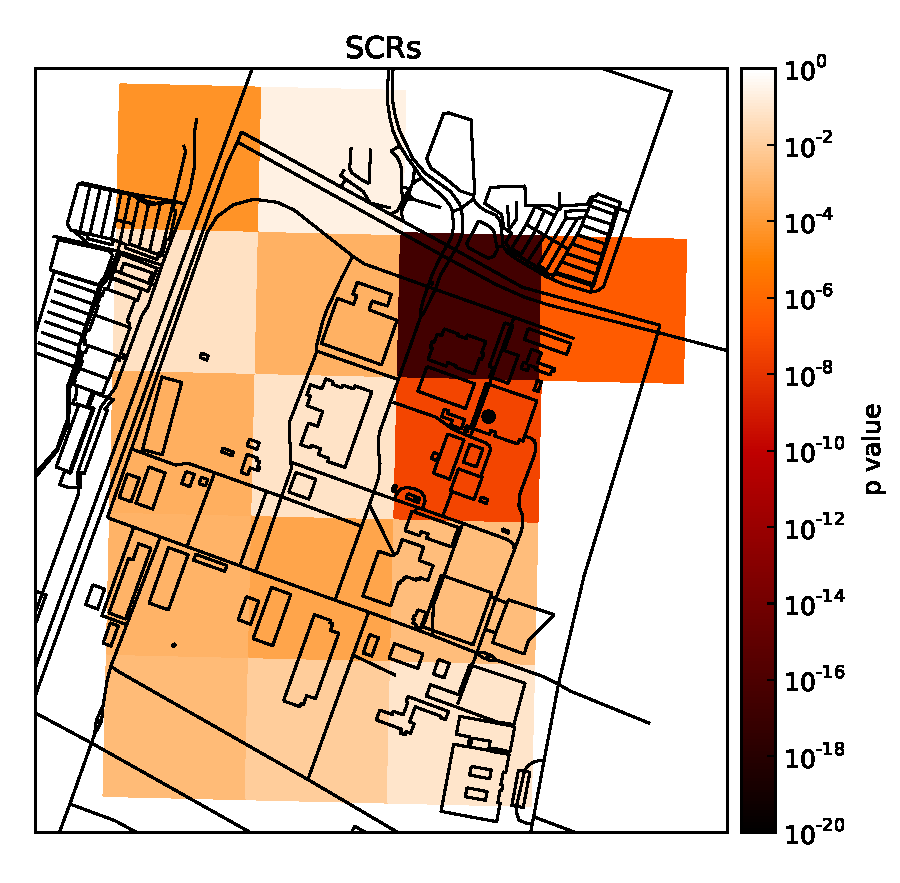
\includegraphics[width=4in]{figures/scr-injected-prc.pdf}
  \caption{Example simulated data from the Pickle Research Campus data described
    in Section~\ref{prcdata}. Here, a 650 mCi cesium-137 radioactive source has
    been injected at the location of the black dot; the resulting spectral
    anomaly is shown in dark red. The detector never traveled closer than 160
    meters to the source.}
  \label{scr-injected-prc}
\end{figure}


\chapter{Experiments}

\section{Pickle Research Campus}\label{prcdata}

We collected a sample dataset between June 22nd and August 10th, 2012 at the
University of Texas's J.J.\ Pickle Research Campus.  To survey the campus, the
system was placed in a golf cart and driven on most work days on irregular
routes. Total observation time amounted to twenty hours in 48 observation runs
containing a total of more than 37,000 individual two-second observations.

\begin{figure}
  \centering
  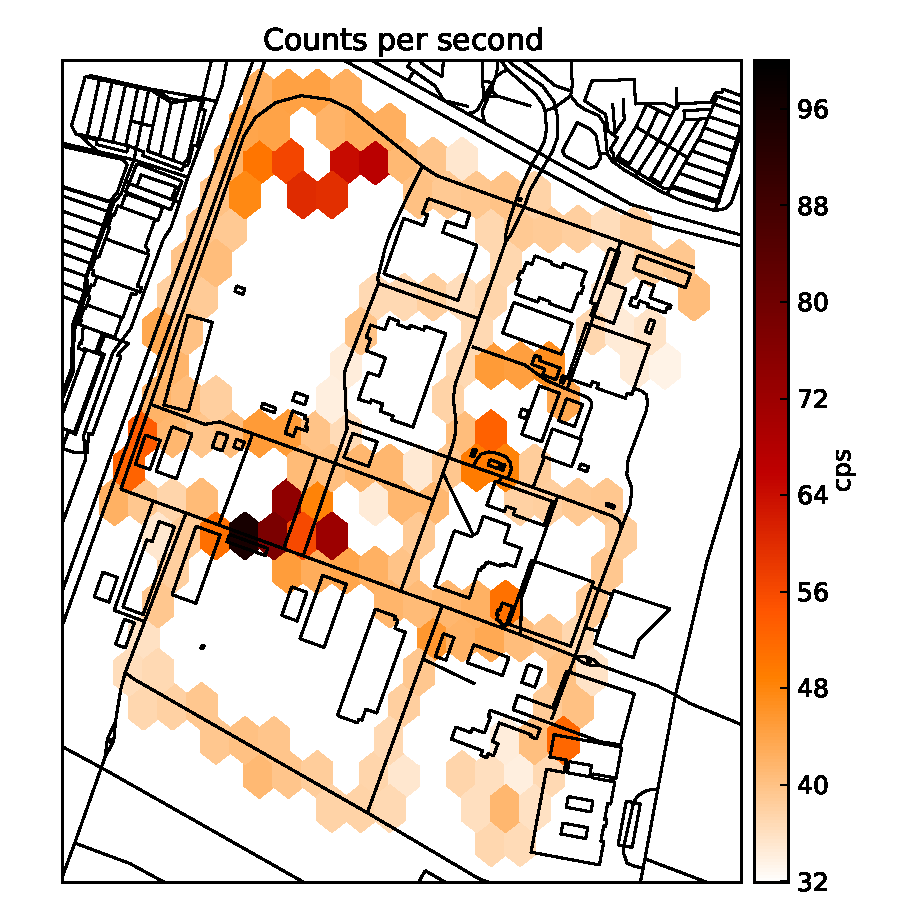
\includegraphics[width=4in]{figures/prc-cps.pdf}
  \caption{A map of J. J. Pickle Research Campus with gamma counts per second
    overlaid.  The campus is approximately 0.33 sq.\ mi., with north
    corresponding to up.  Areas of elevated background include the radioactive
    materials storage facility at the northwest corner and a cluster of large
    brick buildings near central campus.}
  \label{prc-cps}
\end{figure}

The natural gamma background varies spatially and temporally due to many natural
factors.  Our surveys revealed a spatially varying natural background across
Pickle Research Campus. A map of average radiation levels over several weeks is
shown in Fig.\ \ref{prc-cps}. Background activities vary spatially by a factor
of two due to natural and artificial sources.

\subsection{Poisson distribution assumption}

Our algorithmic approach relies on the underlying Poisson distribution of
radiation data.  To test the validity of this assumption, Poisson dispersion
tests were performed on the dataset as a function of spatial scales. The Poisson
dispersion test determines whether a given set of observations could plausibly
have been drawn from the same Poisson distribution \cite{Rao:1956vp}. The test
computes a dispersion parameter \(D\), defined by:
\begin{equation}
D = \frac{\sum_{i=1}^N (x_i - \bar{x})}{\bar{x}},
\end{equation}
where \(\bar{x}\) is the mean of all observations \(x_i\) and \(N\) the total
number of observations. This parameter is \(\chi^2\)-distributed with \((N -
1)\) degrees of freedom. A \(p\) value can be computed for \(D\), indicating the
probability that the observed distribution of values would arise from a
Poisson-distributed random variable. For example, dividing our dataset into
125-meter grid cells, we find that on average, \(p = 0.33\); this falls to \(p =
0.17\) for 250-meter cells, indicating that counts are not perfectly
Poisson-distributed.

To quantify this, the index of dispersion was computed for all grid cells at
various cell sizes. The index of dispersion \(V\) is a measure of the variance
of a distribution, compared to its mean:
\begin{equation}
V = \frac{\sigma^2}{\mu},
\end{equation}
where \(\mu\) is the distribution's mean and \(\sigma^2\) its variance. The
variance of a Poisson distribution equals its mean, so the index of dispersion
is expected to be one. Fig.\ \ref{poisson-dispersion} shows mean indices of
dispersion for various grid cell sizes, demonstrating that smaller cells tend to
have count rate distributions closer to the expected Poisson distribution, as
expected. To account for this, we adjusted the dispersion parameter \(V\) in
Eq.~\ref{vars} to match the mean index of dispersion for grid cells at a
chosen spatial scale.

\begin{figure}
  \centering
  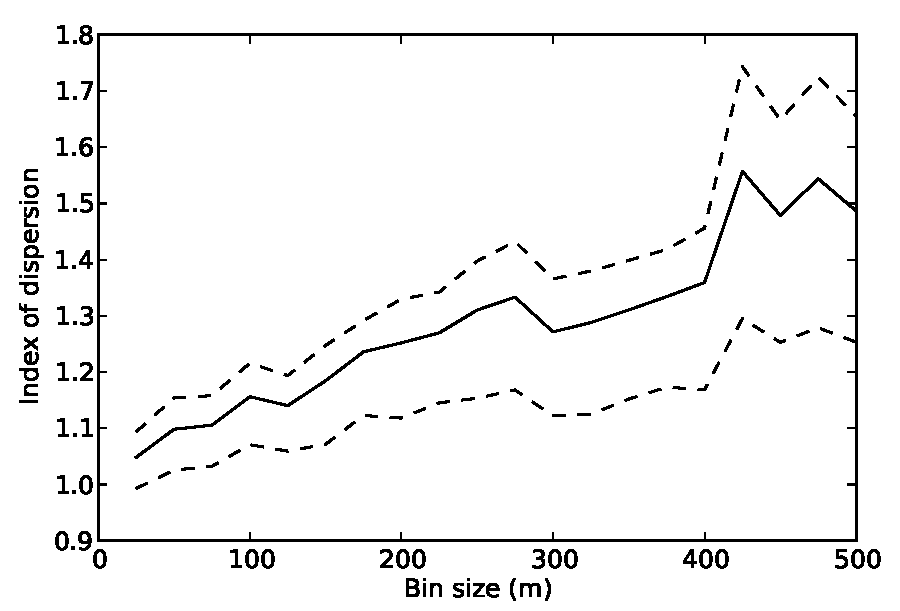
\includegraphics[width=4in]{figures/poisson-dispersion.pdf}
  \caption{Mean, minimum and maximum index of dispersion of counts in each
    energy bin for all grid cells, at specified grid sizes. An index of 1 is
    consistent with a Poisson distribution.  As expected, smaller cells more
    closely match the Poisson distribution, while larger cells have additional
    variance.}
  \label{poisson-dispersion}
\end{figure}

\subsection{Comparing spatial and temporal variation}

Our dataset at the Pickle Research Campus revealed not only spatial but temporal
variation in background. To compare the temporal variation to the spatial
variation, the observation area was divided into grid cells 250 meters on each
side, and each day's set of observations was compared to two or more previous
days using the SCRAM algorithm. Fig.\ \ref{scr-distribution} shows the
distribution of \(D^2\) recorded over several dozen passes through the area. For
comparison, it also plots the \(D^2\) values calculated by comparing each grid
cell's spectrum to a fixed reference cell, rather than comparing it to the same
cell on a previous day.

\begin{figure}
  \centering
  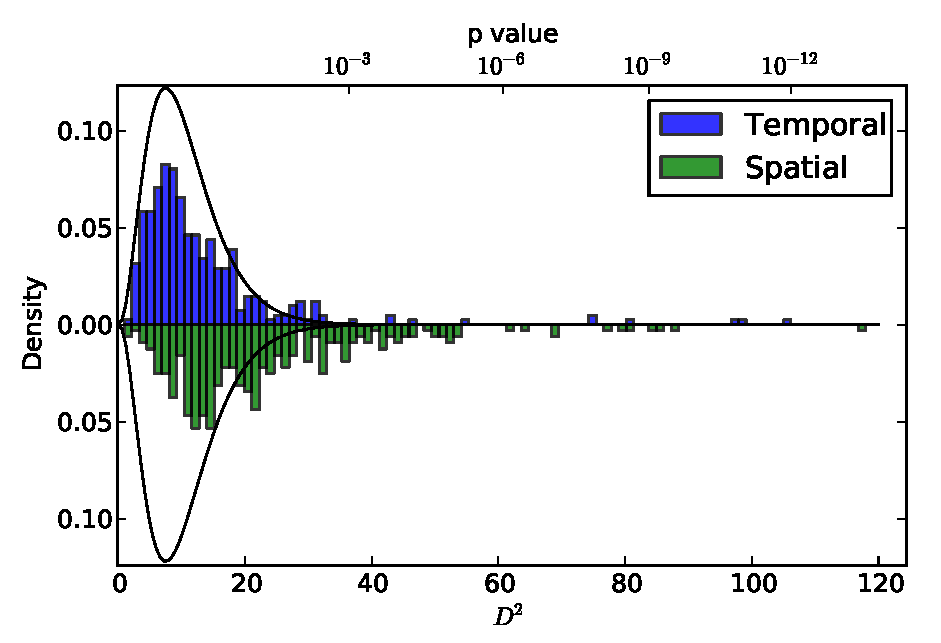
\includegraphics[width=\textwidth]{figures/scr-distributions.pdf}
  \caption{Distribution of the SCR anomaly statistic \(D^2\) in 250-meter grid
    cells in the sample dataset, with a \(\chi^2\) distribution (\(\text{df} =
    7\)) overlaid. The upper histogram is the result of comparing each grid cell
    to the same cell on the previous day; the lower histogram compares each cell
    to a fixed reference cell, showing spatial rather than temporal
    variation. The lower distribution is clearly shifted to the right.}
  \label{scr-distribution}
\end{figure}

The spatial distribution is clearly shifted to the right, indicating that there
is more spatial variance than temporal variance. This validates the assumption
of the SCRAM algorithm that it is best to compare spectral observations to
previous observations made in the same place, rather than observations made at
other locations. In other words, background spectra vary much more spatially
than they do temporally. This suggests that alarm thresholds may be set lower
when using the SCRAM method to perform anomaly mapping, giving higher
sensitivity without increased false alarm rates.

The presence of \(p < 10^{-3}\) anomalies in Fig.~\ref{scr-distribution} is not
unusual. The \(p\)-values are computed under the \(\chi^2\) distribution, which
the data do not follow perfectly. There are, of course, some true variations in
natural background in the data. Also, some spectral comparisons were made with
little data -- because we drove irregular routes, a spatial bin may only contain
a few seconds of data, giving an extremely poor estimate of the spectrum in that
bin.

\section{Blind testing at football games}\label{football}

To validate the detection algorithm it was necessary to perform blind
tests. We needed a large area in which radioactive sources would likely appear
and could be found using the SCRAM technique. University football games meet
these criteria: with 100,000 fans in attendance, it is statistically likely that
at least one or two fans will have recently been exposed to a medical
radioisotope.

First, we took background spectral measurements of the stadium. Measurements
were collected on three separate mornings while the stadium was empty. The
scintillator was carried in a backpack up and down every set of stairs in the
stadium, with a team of three or four walkers operating in shifts.

As seen in Fig.~\ref{stadium-heatmap}, the stadium has a varying natural
background. In particular, the west upper deck appears to have a higher
background activity than the rest of the stadium. The stadium was initially
built with only the lower inner stands, and the west upper deck was constructed
later, with the north and east decks following later. Consequently, different
batches of materials went into the concrete making up the decks, and the
different materials may have different levels of thorium, uranium, and
potassium, the primary contributors to concrete's natural background radiation.

\begin{figure}
  \centering
  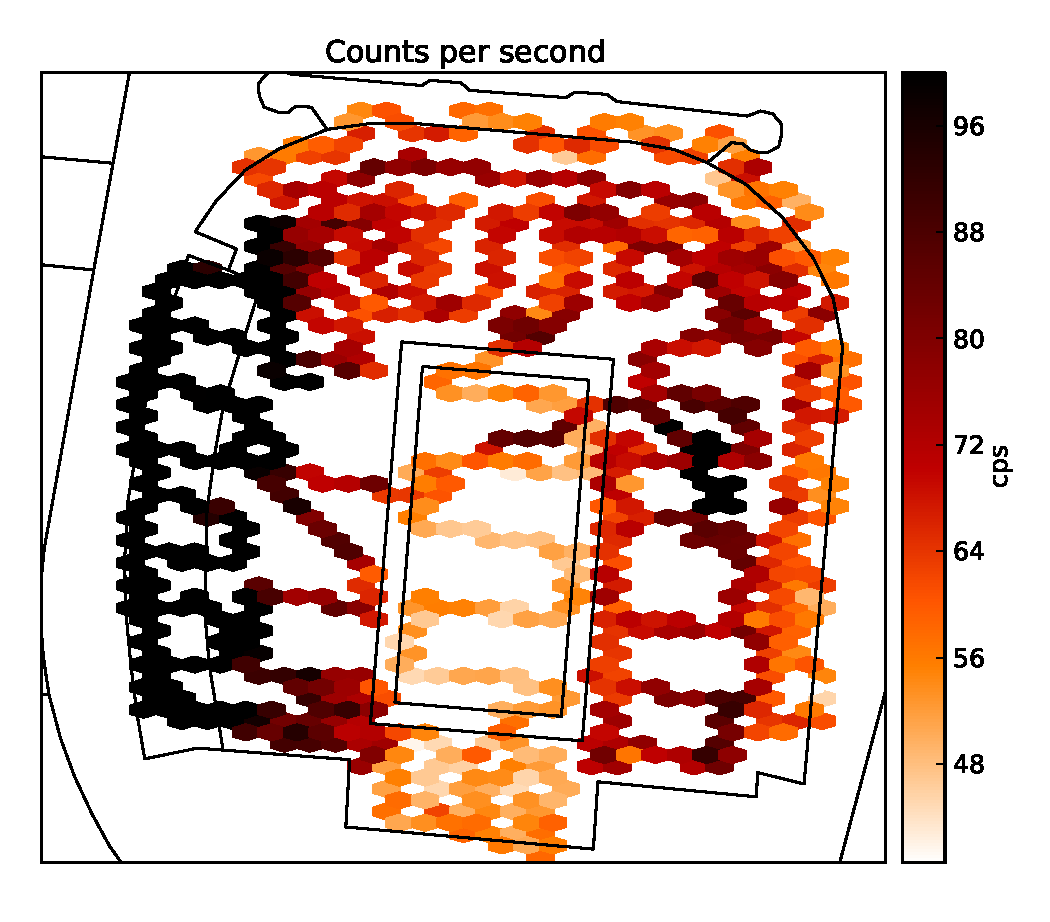
\includegraphics[width=\textwidth]{figures/stadium-heatmap.pdf}
  \caption{An October 1, 2012 background measurement of the stadium. The more
    active area on the left is the west upper deck, which appears to have a
    relatively high natural background radiation. (North is up.) Radiation
    levels are typically \(\approx 10 \,\mu\)R/hr in the west deck, or roughly
    one fiftieth of the dose rate experienced in an airplane traveling at 40,000
    feet.}
  \label{stadium-heatmap}
\end{figure}

This effect can be seen in Fig.~\ref{stadium-concrete}, where spectra from the
east and west decks of the stadium are compared. There are no spectral peaks
unique to the west upper deck; instead, the potassium-40 peak and the low-energy
Compton-scattered region are shifted up, indicating higher levels of
potassium-40 and other natural radioisotopes within the concrete. Levels of
potassium and thorium are known to vary by an order of magnitude within
different samples of concrete, so this is unsurprising.\cite{Ryan:2011wh}

\begin{figure}
  \centering
  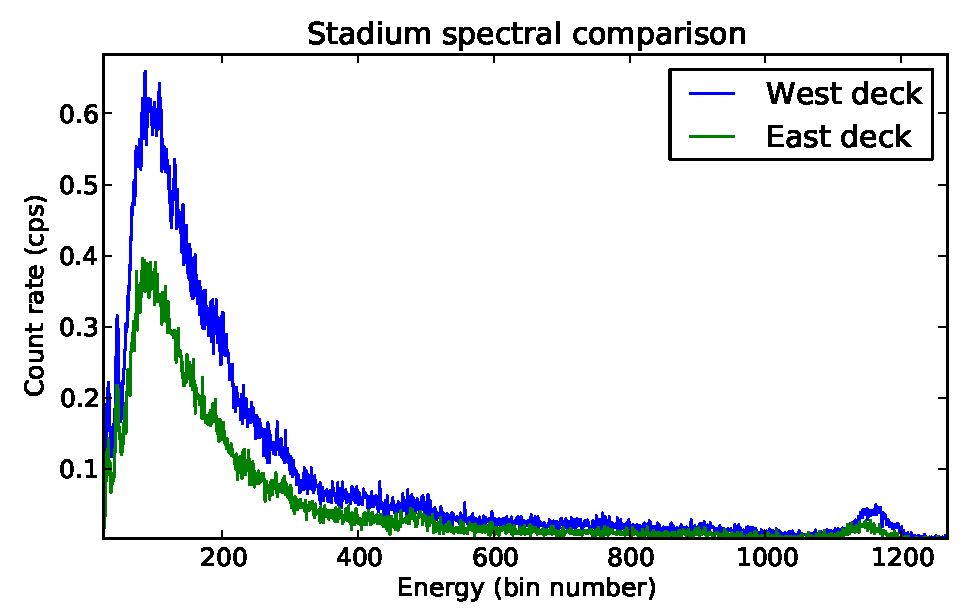
\includegraphics[width=\textwidth]{figures/stadium-concrete.pdf}
  \caption{The west upper deck of the football stadium shows higher source
    activity than the rest of the stadium. Here, the upper spectra is the west
    upper deck, while the lower spectra is the east deck; both spectra are
    normalized to show count rates in counts per second. The west deck evidently
    has more potassium-40 (the peak on the right) and more Compton-scattered
    low-energy gamma activity.}
  \label{stadium-concrete}
\end{figure}

During one background collection run, a calibration problem occurred while
collecting data on the west upper deck. When examining spectra afterwards, it
appeared that the potassium-40 peak had vanished. It appears now this was due to
a shift in calibration while collecting the data; the peak was consequently
``smeared'' across a wide range of energy bins, making it vanish. We did not
remove this data, and so anomaly detection on the west upper deck will tend to
exaggerate spectral changes until sufficient background is collected to hide the
problem. Future work will need to provide automatic energy calibration in
real-time, so spectra are not smeared. It may be possible to calibrate
retrospectively by using known background peaks in the data.

Next, spectra were collected at three football games, each with attendance of
roughly 100,000. While collecting spectra we wore Polimaster personal radiation
detectors, which use a small scintillator to monitor dose rates and provide
alarms when rates suddenly increase. We used these detectors to localize
sources.

We experienced several difficulties collecting data. During our first game, on
October 6, 2012, we were able to detect an iodine-131 source; however, frequent
GPS errors and cabling problems prevented us from recording a complete map of
the stadium. With no real-time way of monitoring the data collection system in
the backpack, we had no way of telling when cables had come unplugged, and we
lost valuable time. We only recorded roughly a quarter of the lower decks, along
with the north and east upper decks.

By the second game on October 20, we had developed a monitoring system that
could be accessed over WiFi from a smartphone. We reinforced cable connections
and were able to record a complete map of the stadium. Two anomalies were
detected, shown in Fig.~\ref{oct20-stadium-scr}. GPS drift was a problem:
despite indicating a good signal lock, the GPS location tended to drift in
random directions when parts of the sky were obscured by overhead
obstacles. Cleaning up this data will be essential for future analysis.

\begin{figure}
  \centering
  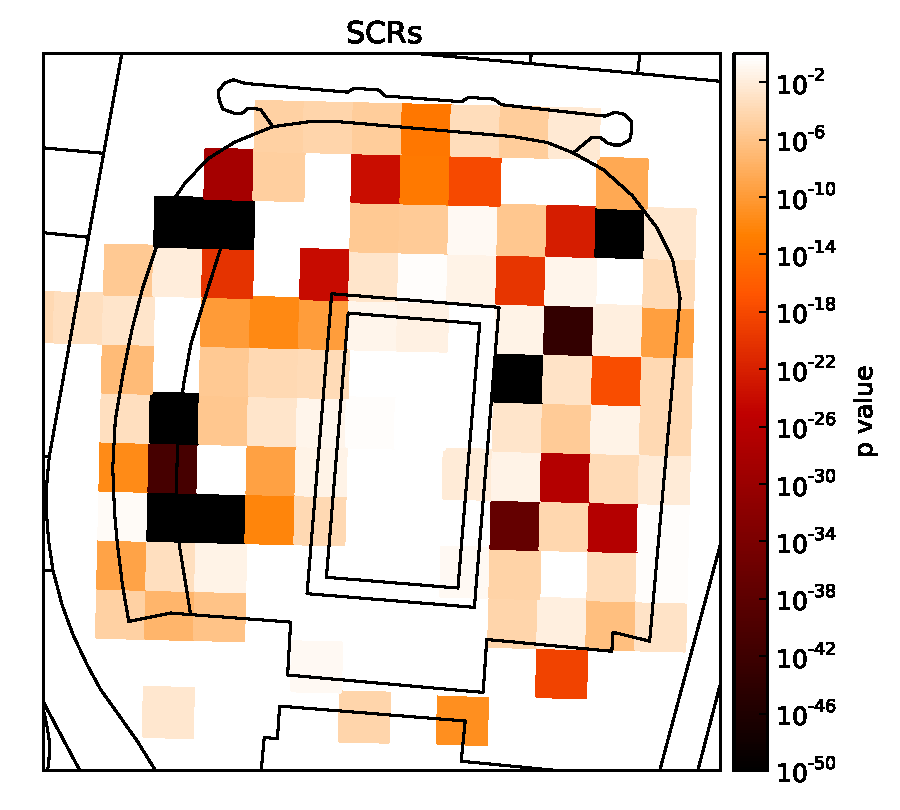
\includegraphics[width=\textwidth]{figures/oct20-stadium-scr.pdf}
  \caption{An SCR map of the stadium on the October 20th run. At the top left
    and lower left, confirmed spectral anomalies are shown. At mid-right is an
    anomaly caused by GPS drift: while investigating the top left anomaly, GPS
    position drifted across the field due to a large overhang blocking the GPS
    signal, and so an anomaly was recorded on the east side of the stadium.}
  \label{oct20-stadium-scr}
\end{figure}

Upon examining the spectra, both spectral anomalies were determined to be
technetium-99m. A representative spectrum is shown in
Fig.~\ref{oct20-spectrum}. One anomaly was easily detectible with our personal
radiation detectors, which alarmed as we walked past; this anomaly was
investigated with a portable identifying spectrometer and confirmed as
technetium-99m. Another was not noticed during the game but appeared in anomaly
maps generated afterward, as the source was smaller or farther away from our
chosen route.

\begin{figure}
  \centering
  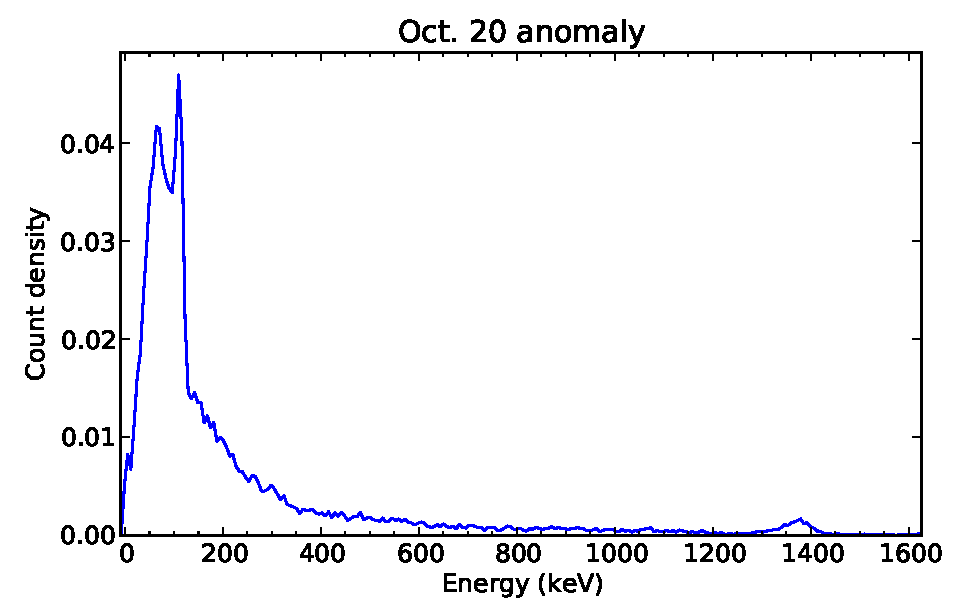
\includegraphics[width=\textwidth]{figures/oct20-spectrum.pdf}
  \caption{A smoothed spectrum recorded during the October 20th data collection
    run at the football stadium. The spectrum is normalized so that its integral
    is one. This appears to be technetium-99m from a medical patient inside the
    stadium. Environmental Health and Safety verified this with a portable
    identifying spectrometer.}
  \label{oct20-spectrum}
\end{figure}

Another game was recorded on November 10, with complete coverage of the stadium
again achieved. Two Tc-99m anomalies were again observed, one with an activity
100 times greater than background at a distance of less than a meter.

These tests demonstrated the utility of the SCRAM system for the monitoring of
public events and large areas. The system was able to accurately identify
spectral anomalies caused by medical radioisotopes, allowing further
investigation by Environmental Health and Safety or the University of Texas
Police Department. Some false positive results were produced, and the causes of
these will need to be investigated. One potential cause of false positives is
the comparison of spectra from consecutive games: if a medical source is present
during one game but missing during the next, this may be counted as an
anomaly. A principled system to exclude anomalous data from background
measurements will be required.

\section{Minimum detectable sources}

To test the performance of the SCRAM algorithm, we performed a simulation to
calculate the minimum detectable radioactive source size at a variety of
distances. We selected a straight stretch of road on the northwest corner of the
Pickle Research Campus and simulated the injection of a cesium-137 source at
various distances from the road into the collected background data.

To choose our alarm threshold, we used the anomaly statistics distribution data
shown in Fig.~\ref{scr-distribution}, selecting a threshold which gives a 1\%
false-alarm rate in our example dataset. For temporal comparisons of spectra,
this threshold is \(D_A^2 = 83\), while for purely spatial comparisons the
result is \(D_A^2 = 113\). We computed the minimum detectable source sizes for
both thresholds, and the results are given in Fig.~\ref{minimum-detectable}.

\begin{figure}
  \centering
  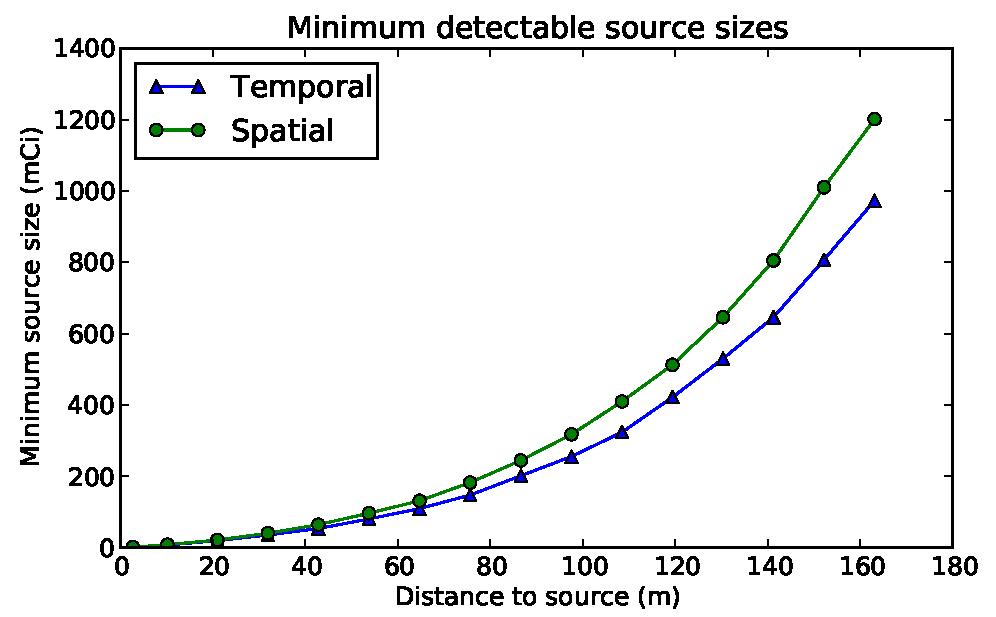
\includegraphics[width=\textwidth]{figures/minimum-detectable.pdf}
  \caption{The minimum detectable cesium-137 source sizes at various distances
    away from the detector's path, using both temporal and spatial comparisons
    of spectra. Total observation time was 136 seconds.}
  \label{minimum-detectable}
\end{figure}

These results show that taking advantage of the exact prior background spectrum
at each location leads to better detection performance by approximately 20\%. Of
course, smaller sources would be detectable with a much larger scintillator or
with a much longer observation time. It will also be necessary to validate these
results experimentally.

\section{Bus route simulation}

To evaluate the feasibility of using the SCRAM algorithm with public transit
vehicles to monitor a wide area, we performed a simulation using Capital Metro
bus routes in downtown Austin, Texas. The results demonstrated the feasibility
of the SCRAM method for real-time monitoring of a wide area, such as the
downtown of a city.

Bus routes were extracted from shapefiles made available by Capital
Metro.\cite{capmetro} We selected only those routes which passed through
downtown Austin multiple times daily, excluding infrequent express routes; the
resulting routes are shown in Fig.~\ref{downtown-map}, along with a map of
Austin.

\begin{figure}
  \centering
  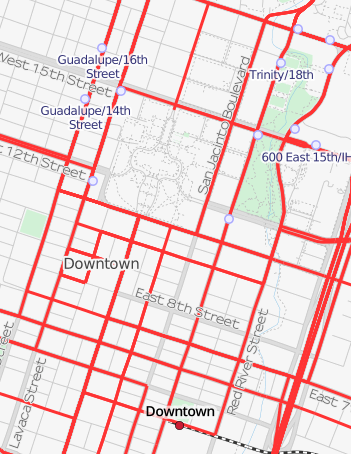
\includegraphics[width=0.5\textwidth]{figures/downtown-transport-map.png}
  \caption{A map of downtown Austin bus routes. Data provided by
    OpenStreetMap,\cite{osm} with rendered map by Andy Allan.}
  \label{downtown-map}
\end{figure}

To simulate observations made by passing buses, a simulated bus traversed each
route defined in the shapefiles. The shapefiles define a route as a series of
connected points; we simulated a bus which stopped at each point for ten
seconds. Given the typical spacing between points of 115 meters, this comes out
to roughly 25 miles per hour average speed for each bus. Each bus was modeled as
traveling its route exactly once. Additional simulation runs could be performed
to have buses make multiple passes.

Background radiation for the area of downtown Austin was simulated. A
representative background spectrum was selected from the Pickle Research Campus
data and simulated at a constant activity of 50 counts per second (plus random
Poisson variation) across the observation region; a 1 Ci point source with a
spectrum taken from Pickle Research Campus was simulated downtown; and a 30 Ci
source with a spectrum taken from a brick building at Pickle Research Campus was
placed at the Texas State Capitol, simulating the higher activity from its
granite construction.

For background observations, twelve separate passes were simulated with the
aforementioned background sources. A 3.5 Ci cesium-137 source was then injected
at the site of the Texas State Capitol at a point which is 240 meters from the
nearest bus routes. At this distance, the source contributes roughly 10 counts
per second to the normal background rate of 50 cps. Using a simple personal
radiation detector which looks for an anomaly in total count rates several
standard deviations above background, this anomaly would not be detected.

Twelve bus passes were made with the injected source, producing an anomaly map
shown in Fig.~\ref{downtown-scrs}.

\begin{figure}
  \centering
  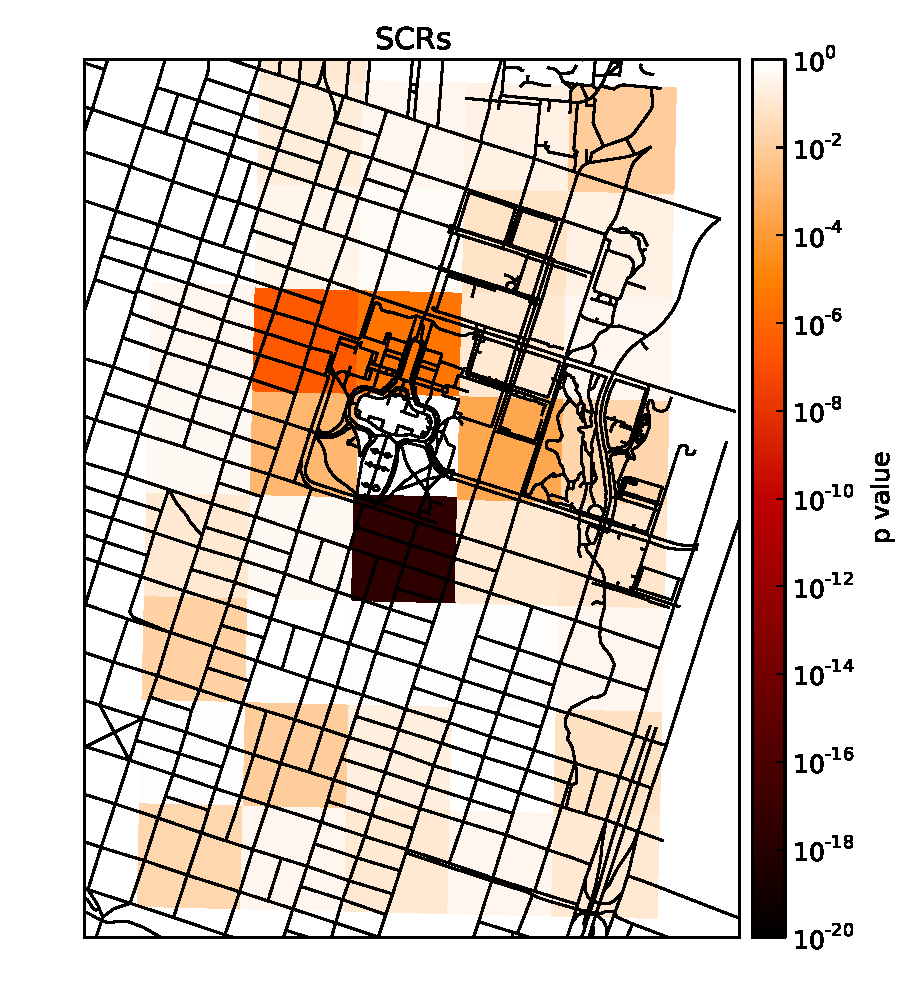
\includegraphics[width=0.8\textwidth]{figures/downtown-injected-scrs.pdf}
  \caption{A 3.5 Ci cesium-137 source has been injected at the site of the Texas
    State Capitol in this image. The nearest bus routes are shown in
    Fig.~\ref{downtown-map}, and are at least 240 meters away from the
    source. The anomaly was detected nevertheless.}
  \label{downtown-scrs}
\end{figure}

This simulation demonstrates the feasibility of the SCRAM system for wide-area
surveillance using public vehicles. Because buses pass through downtown Austin
frequently, many observations can be collected and small anomalies detected
relatively quickly.

In the future we hope to collect accurate wide-area data of downtown Austin or
another area to enable better simulations. Also, the simulation system does not
account for attenuation caused by the presence of large buildings in Austin;
more detailed simulation and experimental work would be needed to determine
detection capabilities when sources are shielded by buildings, vehicles, or
crowds.


\chapter{Poisson kriging}\label{kriging}

The methods presented so far are effective, but they do not take advantage of
some of the known structure in the data. For example, each spatial bin is
treated entirely independently, using only background observations collected
inside the bin. However, we know that the background should only vary slowly in
space, so it should be possible to use other nearby observations to improve our
estimate of the background spectrum.

This has some advantages over the SCRAM method, which ignored all observations
outside a spatial bin, and consequently suffered a tradeoff: large spatial bins
have plenty of data with which to characterize the background spectrum, but
point sources within those bins will be aggregated together with other data and
``diluted.'' If we build a model which understands the spatial correlation of
the data, however, it will be able to produce an accurate background estimate
while also localizing sources to very small bins.

One method to achieve this is kriging. Kriging is a geostatistical method which
models each datapoint as an observation of some random field with an unknown
mean and variance; values of the field at different points are related with a
covariance function which is a function of distance. (Covariance functions may
depend on more than distance if the field is not isotropic -- for instance, if
there is a stronger north-south correlation than east-west.)

Mathematically, this model is
\begin{equation}
  Z(\mathbf{s}) = S(\mathbf{s}) + \epsilon(\mathbf{s}), \qquad \mathbf{s} \in D,
\end{equation} 
where \(Z(\cdot)\) is the observed data as a function of \(\mathbf{s}\), which
indexes locations in some domain \(D\), \(S(\cdot)\) is the underlying random
function, and \(\epsilon(\cdot)\) is some measurement error.\cite{Cressie}

Kriging is a process to predict either \(Z(\cdot)\) or \(S(\cdot)\) at some new
location using data \(Z(\mathbf{s}_1),\ldots,Z(\mathbf{s}_n)\) observed at
locations \(\mathbf{s}_1,\ldots,\mathbf{s}_n\), while also providing estimates
of the prediction variance at the new location. Kriging seeks to minimize the
mean squared error of the predictions through smoothing. Kriging methods
generally assume that the underlying data are Gaussian; a full account of these
traditional methods can be found in \cite{Cressie}.

In our case, however, the underlying data (count rates) are not
Gaussian. Instead, we assume that gamma ray count rates are
Poisson-distributed. Also, observations (numbers of counts) depend not only on
the underlying mean but the amount of time spent observing at each point, and
prediction variances should take this into account: predictions made in areas
with much longer observations should have smaller prediction variances than
those made in areas with short observations.

The methods of Poisson kriging have previously been developed for other
purposes, such as the estimation of whale populations in the Mediterranean Sea
using data from observers on ferries and cargo ships,\cite{Monestiez:2006jp} or
mapping of disease risks using reports from doctors.\cite{Goovaerts:2008dj} A
brief overview follows.

It is assumed that observations \(Z(\cdot)\) are dependent on some underlying
mean count rate \(Y(\cdot)\) along with \(t(\cdot)\), the amount of time spent
counting at the given location. Statistically,
\begin{equation}
  Z(\mathbf{s}) | Y(\mathbf{s}) \sim \text{Poisson}(t(\mathbf{s}) Y(\mathbf{s})),
\end{equation}
where \(Y(\cdot)\) is a second-order stationary positive random field with mean
\(m\), variance \(\sigma_Y^2\), and covariance function \(C(\mathbf{s},
\mathbf{s'})\) which is dependent only on the distance \(||\mathbf{s} -
\mathbf{s'}||\).

The covariance function \(C\) is related to the variogram \(\gamma_Y\) by the
relation 
\begin{equation}\label{var-covar}
  C(\mathbf{s}, \mathbf{s'}) = \sigma_Y^2 - \gamma_Y (\mathbf{s},
  \mathbf{s'}).
\end{equation}
This relationship will be useful later.

Our goal, then, is to predict \(Y(\cdot)\) using our observations
\(Z(\mathbf{s}_1),\ldots,Z(\mathbf{s}_n)\). For a full derivation of the
procedure, see \cite{Monestiez:2006jp}. We assume that our prediction \(\hat Y\)
is simply some weighted average of the observations:

\begin{equation}
  \hat{Y}(\mathbf{s}_0) = \sum_{\alpha=1}^n \lambda_\alpha
  \frac{Z(\mathbf{s}_\alpha)}{t(\mathbf{s}_\alpha)}
\end{equation}

We must simply determine the weights \(\lambda_\alpha\). We then seek to
minimize the mean squared error of prediction and constrain \(\lambda_\alpha\)
so the result is an unbiased estimator of \(Y(\mathbf{s}_0)\). The result is a
system of \(n+1\) linear equations which must be solved for \(\lambda\):
\begin{align}
  \sum_{\beta=1}^n \lambda_\beta C(\mathbf{s}_\alpha, \mathbf{s}_\beta) +
  \lambda_\alpha \frac{m}{t(\mathbf{s}_\alpha)} + \mu &= C(\mathbf{s}_\alpha,
  \mathbf{s}_0)\qquad \text{for } \alpha = 1, \ldots, n\\
  \sum_{\alpha=1}^n \lambda_\alpha &= 1
\end{align}
Here \(\mu\) is a Lagrange multiplier used to apply the constraint on
\(\lambda_\alpha\). The system can be re-expressed in matrix form, allowing it
to be solved much more easily with modern linear algebra software packages. In
short,
\begin{equation}\label{krige-system}
  \lambda_0 = \Gamma_0^{-1} C_0,
\end{equation}
where
\begin{align}
  \lambda_0 &= (\lambda_1, \ldots, \lambda_n, \mu)^T\\
  C_0 &= (C(\mathbf{s}_0, \mathbf{s}_1),\ldots, C(\mathbf{s}_0, \mathbf{s}_n),
  1)^T\\
  \Gamma_0 &= \begin{cases}
C(\mathbf{s}_i, \mathbf{s}_j) & i=1,\ldots,n,\; j=1,\ldots n, \; i\neq j\\
C(\mathbf{s}_i, \mathbf{s}_j) + \frac{m}{t(\mathbf{s}_j)} & i=j, \; i<n+1,\; j<n+1\\
1 & i = n+1,\; j=1,\ldots,n\\
0 & i=n+1, \; j=n+1\\
\end{cases}
\end{align}

Here, \(m\) is estimated from the data as a weighted average of count rates
(\(Z(\cdot)/t(\cdot)\)), where the weights correspond to the observation
times. % todo: formalize this

Prediction variances fall out of this system as well:
\begin{equation}\label{prediction-variance}
\text{var}(\hat Y_0 - Y_0) = \sigma_Y^2 - \sum_{\alpha = 1}^n \lambda_\alpha
C(\mathbf{s}_\alpha, \mathbf{s}_0)
\end{equation}

As one would expect, prediction variances are smallest in areas where the most
data has been collected.

\section{Efficient computation for multiple simultaneous variables}

We are interested in performing kriging to predict spectra. This suggests we
will be solving several simultaneous kriging systems: if we divide the spectrum
into energy bins, we must krige the count rates in each bin separately. (There
is inevitably covariance between the count rates in separate bins; we neglect
this covariance. Our methods can be extended to support cokriging later, should
it become necessary.)

It would be computationally expensive to recompute the matrix \(\Gamma_0\) for
each variable. Fortunately, the diagonal entries are the only ones that differ
-- because all spectral bins are measured simultaneously, the off-diagonal
entries referring to covariance should be identical. The matrix can be computed
once without the additional term on the diagonals and saved for
reuse. Similarly, \(C_0\) will be the same for each kriged variable.

We also need to make predictions at more than one point; we may choose to make
predictions on a grid or in particular regions of interest, and so we'd like to
repeatedly solve the system with different values of \(\mathbf{s}_0\). This
would be slow, because repeatedly solving Eq.~\ref{krige-system} for different
values of \(C_0\) would be very slow. Instead, we compute the LU factorization
of \(\Gamma^0\) once, and use the LU factorized form to solve
Eq.~\ref{krige-system} at each prediction point.

This is much faster. Matrix inversion is an \(O(n^3)\) operation, where \(n\) is
the dimension of the matrix; LU factorization and solving are only \(O(n^2)\)
operations. Instead of an \(O(n^3)\) operation for each predicted point, we only
need an \(O(n^2)\) operation. This is still slower than we'd like, but the
system is at least practical.

\section{Estimating the variogram}

The variogram \(\gamma_Y\) must somehow be estimated from the data so our model
understands the relationship between observations taken at various distances. We
use a weighted variogram estimator which accounts for the different observation
times of each point \cite{Monestiez:2006jp}:
\begin{equation}
  \hat \gamma_Y (h) = \frac{1}{2N(h)} \sum_{\alpha, \beta} \left(
    \frac{t(\mathbf{s}_\alpha) t(\mathbf{s}_\beta)}{t(\mathbf{s}_\alpha) +
      t(\mathbf{s}_\beta)} \left(
      \frac{Z(\mathbf{s}_\alpha)}{t(\mathbf{s}_\alpha)} -
      \frac{Z(\mathbf{s}_\beta)}{t(\mathbf{s}_\beta)} \right)^2 - \hat m \right)
  I_{d_{\alpha \beta} \approx h},
\end{equation}
where
\begin{equation}
N(h) = \sum_{\alpha, \beta}  \frac{t(\mathbf{s}_\alpha) t(\mathbf{s}_\beta)}{t(\mathbf{s}_\alpha) +
      t(\mathbf{s}_\beta)} I_{d_{\alpha \beta} \approx h},
\end{equation}
while \(h\) is the chosen distance and \(I_{d_{\alpha \beta} \approx h}\) the
indicator function which is 1 when \(\alpha\) and \(\beta\) are roughly a
distance \(h\) apart and 0 otherwise.

Because this estimator requires calculating the distance between every pair of
observations, it requires \(O(n^2)\) operations to complete, where \(n\) is the
number of observations. This rapidly becomes impractical for datasets of any
nontrivial size. To simplify the problem, data was aggregated in twenty-meter
spatial bins, with all data within each bin being treated as a single
observation taken at the bin's centroid.

Once the variogram is estimated at a range of distances, a model variogram
function can be fit to the estimated values using nonlinear least squares. We
chose a stable variogram model of the form
\begin{equation}\label{var-model}
  \gamma_Y(h) = c\left(1 - \exp \left(- \left(\frac{h}{a}\right)^d \right)\right),
\end{equation}
with \(c\), \(a\) and \(d\) being tunable parameters that control the behavior
of the variogram at various distances, and \(0 < d \leq 2\).\cite{Chiles} (We
use a model such as this rather than any arbitrary function fit to the data
because an arbitrary function will most likely not be positive definite, which
is a requirement for valid variograms.)

As an example, the empirical variogram for the stadium data (see
Ch.~\ref{football}) is shown in Fig.~\ref{stadium-variogram} along with the fit
variogram model. In this case, the fit returned \(c=802\), \(a=111.9\),
\(d=0.846\).

\begin{figure}
  \centering
  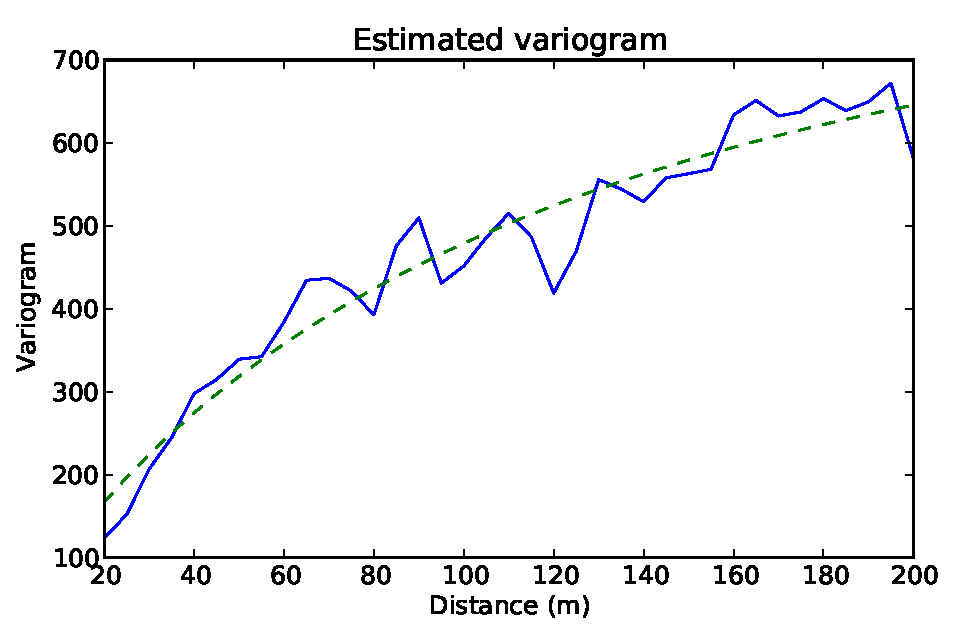
\includegraphics[width=\textwidth]{figures/stadium-variogram.pdf}
  \caption{An empirically estimated variogram model for \(h\) ranging from 20 to
    200 meters, in 5-meter increments, along with the fit model (dashed
    line). After 200 meters, the number of data points available to estimate the
    variogram becomes too small for reliable estimation.}
  \label{stadium-variogram}
\end{figure}

Since the kriging equations are expressed in terms of the covariance, we must
make use of Eq.~\ref{var-covar} to turn the estimated variogram into an
estimated covariance. This requires estimating \(\sigma_Y^2\), the variance of
the underlying random field. (The equations may be re-expressed in terms of the
variogram, but this also requires \(\sigma_Y^2\).)

To do so, we restate Eq.~\ref{var-covar} in terms of \(h\), the distance between
\(\mathbf{s}\) and \(\mathbf{s'}\), and take the limit:
\begin{equation}
  \lim_{h\to\infty} C(h) = \lim_{h\to\infty} \sigma_Y^2 - \gamma_Y (h)
\end{equation}
Of course, the covariance function goes to zero at infinite distance, under the
assumption of ergodicity. So we find that
\begin{equation}
\sigma_Y^2 = \lim_{h\to\infty} \gamma_Y(h),
\end{equation}
which is \(c\) in our chosen variogram model (Eq.~\ref{var-model}).

\section{Producing count rate maps}

A first step to implementing kriging for anomaly detection is to produce simple
maps of measured count rates. Python code implementing the above kriging system
was implemented using the SciPy library, which uses the LAPACK fast linear
algebra library to perform its operations. 

No matter how powerful the linear algebra library, it is still computationally
infeasible to solve Eq.~\ref{krige-system} on a consumer laptop when there are
several thousand data points to krige. We can give up some resolution and
instead aggregate our data into small spatial bins. In each spatial bin,
observations are summed and the total observation time computed; the resulting
aggregate data is then assigned the location of the ``center of mass''
(centroid) of the observations.

On datasets such as our Pickle Research Campus example data, a 20-meter bin
spacing produces reasonable results without requiring more than a minute or two
of calculation.

The kriging system is then used to create predicted count rates and variances
for each spatial grid point, and a contour plot made of the result. An example
is plotted in Fig.~\ref{prc-cps-contour} and Fig.~\ref{prc-cps-var-contour}.

\begin{figure}
  \centering
  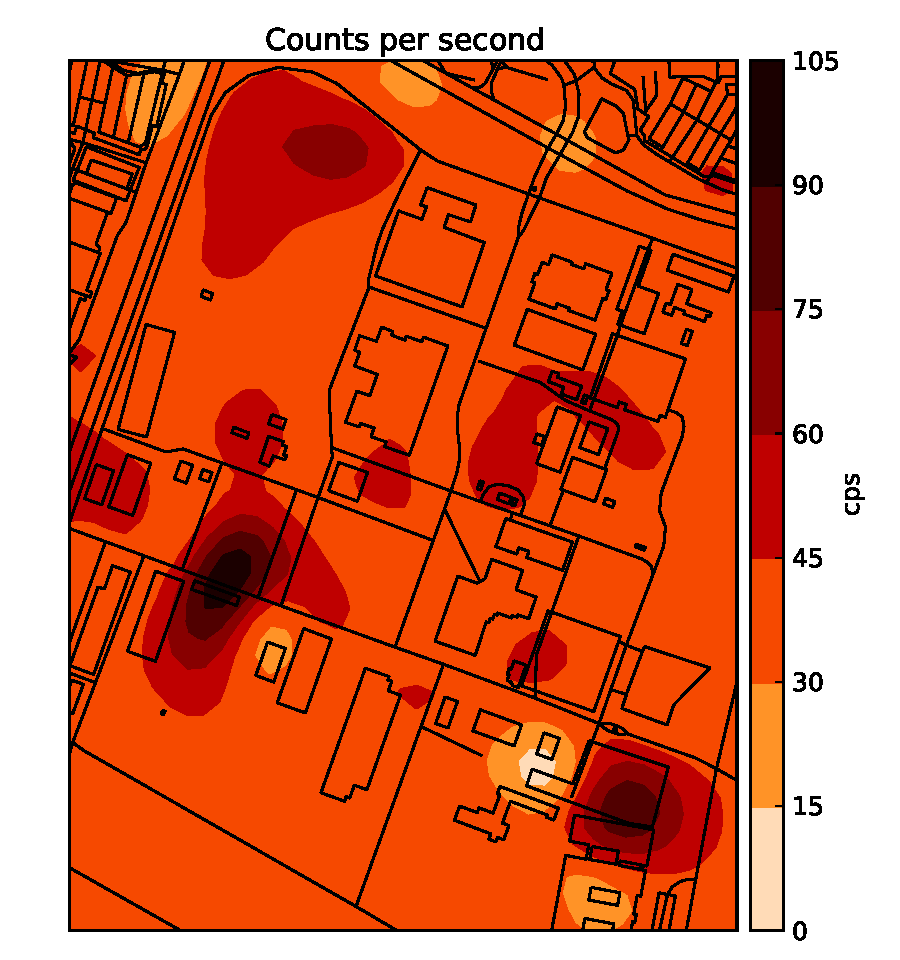
\includegraphics[width=0.8\textwidth]{figures/prc-cps-contour.pdf}
  \caption{Kriged mean count rates across the Pickle Research Campus during July
    2012. Compare against Fig.~\ref{prc-cps}. The same radioactive sources are visible.}
  \label{prc-cps-contour}
\end{figure}

\begin{figure}
  \centering
  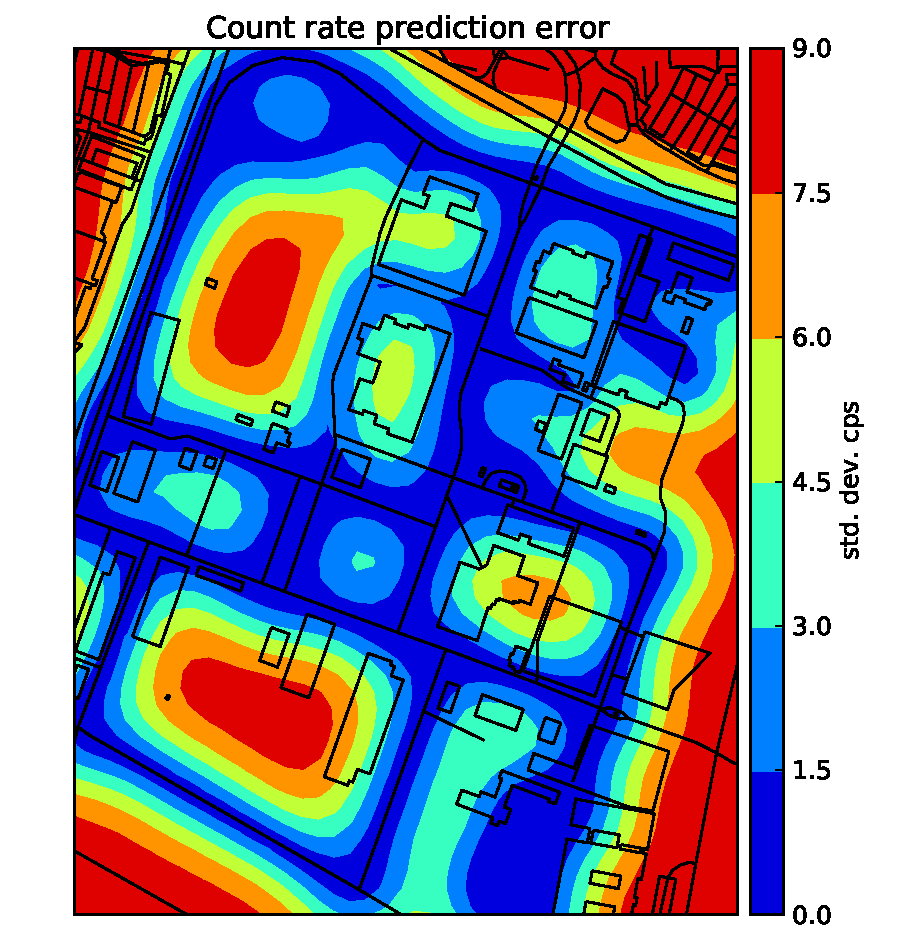
\includegraphics[width=0.8\textwidth]{figures/prc-cps-var-contour.pdf}
  \caption{Kriged prediction errors across the Pickle Research Campus in
    July 2012.}
  \label{prc-cps-var-contour}
\end{figure}

\section{Kriging anomaly detection}

\subsection{Anomaly mapping procedure}\label{krige-anomaly-mapping}

Anomaly detection emerges from kriging naturally. With Poisson kriging, we have
a system for mapping gamma count rates and producing predictions, with attached
variances, at any location. We may compare these predictions with new data to
see whether the new data is consistent with the past. In outline form, our
strategy is as follows:

\begin{enumerate}
  \item Collect a series of background observations in a region.
  \item Divide the region into spatial bins, as before, and perform kriging on
    the background observations to produce a prediction and matching prediction
    variance.
  \item Aggregate the new observations into spatial bins and compare the
    spectrum in each bin to the kriged prediction for that bin, producing a
    \(p\) value for the spectral difference.
  \item Produce a map of the \(p\) values.
\end{enumerate}

The first two steps are straightforward. But to perform steps 3 and 4, we need
an anomaly statistic.

\subsection{Count rate anomaly statistics}

Kriging provides us predictions and their prediction variance, which we must use
to determine if the new observations are consistent with the past. If we want
the predictive distribution of \(Z(\mathbf{s})\), the counts observed at some
new observation point, using the kriged prediction \(\hat Y(\mathbf{s})\), we
have:
\begin{align}
  Z(\mathbf{s}) | \hat Y(\mathbf{s}) t(\mathbf{s}) &\sim \text{Poisson}(\hat Y(\mathbf{s})
  t(\mathbf{s}))\\
  \hat Y(\mathbf{s}) t(\mathbf{s}) &\sim \text{Gamma}(a, (1-b)/b),
\end{align}
where \(t(\mathbf{s})\) is the observation time at the new point, and \(a\) and
\(b\) are chosen to match the mean and variance of the gamma distribution with
the prediction and prediction variance. In this case,
\(E[Y(\mathbf{s})t(\mathbf{s})] = t(\mathbf{s}) E[Y(\mathbf{s})]\) and
\(\text{var}(Y(\mathbf{s})t(\mathbf{s})) = t(\mathbf{s})^2
\sigma_Y^2\), so:
\begin{align}
  a &= \frac{\hat Y^2}{\sigma_{\hat Y}^2}\\
  b &= \frac{t(\mathbf{s}) \sigma_{\hat Y}^2}{\hat Y + t(\mathbf{s}) \sigma_{\hat Y}^2}.
\end{align}

Here \(\sigma_{\hat Y}^2\) is the prediction variance estimated by the kriging
procedure and \(\hat Y\) the predicted mean. With this information we can
compute the posterior predictive distribution of \(Z(\mathbf{s})\), our new
observation. For ease of integration, I substitute
\(x=Y(\mathbf{s})t(\mathbf{s})\):
\begin{equation}
P(Z(\mathbf{s})) = \int_0^\infty P(Z(\mathbf{s})|x) P(x) \, dx
\end{equation}
This integral is analytically tractable, and turns out to be a
negative binomial distribution with parameters \(a\) and \(b\):
\begin{equation}\label{post-predictive}
  Z(\mathbf{s}) \sim \text{NB}(a,b)
\end{equation}
We can use this to easily compute \(p\) values for our observed \(Z\), comparing
it to the predictions we derive from our background data.

\subsection{Detecting spectral anomalies}\label{spectral-anomaly}

The SCRAM algorithm aims to detect differences in spectral shape rather than
overall count rate, and we would like to replicate that behavior. To do this, we
divide the spectrum into bins as before, and krige the count rate in each bin
independently. (Cokriging may be more appropriate, because count rates in
separate energy bins are likely to be correlated; however, we did not explore
cokriging here.)  We then perform the count rate detection algorithm on each
energy bin in the spectrum.

Suppose there are \(n\) energy bins. We would like to know if any single bin has
an abnormally high count rate; to do this, we take the minimum \(p\) value out
of the \(n\) computed. Because \(p\) values are uniformly distributed on the
\((0,1)\) interval, the minimum of \(n\) is distributed as
\(\text{Beta}(1,n)\).\cite{David} Consequently we can compute an anomaly
statistic across all \(n\) bins by using the density of the beta distribution.

\subsection{Choosing an alarm threshold}

We will need to use a procedure to control false alarms. Typical hypothesis
testing provides bounds on the familywise error rate, which answers the question
``If there are no anomalies, how frequently will I falsely detect an anomaly?''
The simplest method is the Bonferroni correction, in which we set our
statistical significance criterion to be \(p < \alpha/n\), where \(n\) is the
number of tests performed. This method limits our statistical power, requiring a
high threshold of significance, though other more sophisticated techniques exist
with greater power.\cite{Holm:1979ws}

In a practical sense, though, we are not interested in the familywise error
rate. Operators of a radiation anomaly detection system are more concerned with
the false discovery rate: what proportion of alarms are false alarms?

The difference between familywise error rate and false discovery rate can be
seen by example. Suppose we test for anomalies each day, but true anomalies only
appear once every 1,000 days. If we control for a 1\% familywise error rate and
detect every single true anomaly, there will be 10 false positives and one true
positive.

In practical use, this is highly inconvenient. A system with too many false
positives is a system that will be ignored; each false positive incurs a cost to
investigate and dismiss. We would prefer the false discovery rate to be much
lower.

(Of course, there will be other sources of false positives beyond statistical
error: medical radioisotopes in recently treated patients, the transport of
industrial sources, and so on. Many of these can be mitigated with other
techniques, such as spectral analysis to determine the type of radioactive
source detected.)

We use the Benjamini-Hochberg procedure to control false discovery
rate.\cite{Benjamini:1995ws} We compute \(p\) values at many spatial points
following the procedure in Section~\ref{krige-anomaly-mapping}. Let the \(N\)
\(p\) values be denoted by \(P_{(1)}, P_{(2)}, \ldots, P_{(n)}\), sorted in
ascending order. Then, let \(k\) be the largest \(i\) such that
\begin{equation}
P_{(i)} \leq \frac{i}{N} q
\end{equation}
where \(q\) is the false discovery rate desired. We may reject all the
hypotheses where \(1 \leq i \leq k\). This is guaranteed to maintain a false
discovery rate of \(q\) or less.

This procedure will have higher statistical power than a procedure designed to
meet a certain false discovery rate goal while producing more useful results. In
one example case, we searched for anomalies in a map containing 138 kriged
points, most of which were true anomalies. Had we chosen to target an overall
false-positive rate of \(\alpha = 0.05\) using the Bonferroni correction, we
would have required \(p < 3.6\times 10^{-4}\); targeting \(q=0.05\), a much more
useful goal, allows searching for \(p < 0.12\), a factor of 319 difference. The
anomalies were successfully detected.

In another test, we searched for anomalies in a map containing 116 kriged points
in which there were no known true anomalies. The \(p\) criterion from the
Benjamini-Hochberg procedure was 5 times higher than that from the Bonferroni
correction, and even then, the system correctly reported no anomalies. One can
see how the Benjamini-Hochberg procedure adapts, choosing different criteria
based on the distribution of \(p\) values in the data.

Variations on the Benjamini-Hochberg procedure have been developed for the case
where the test statistics are dependent, which is the case
here.\cite{Benjamini:2001ho} The original procedure still works quite well in
this case, however, so we did not explore alternatives which account for the
dependency. Future work may seek to characterize the spatial dependence in
anomaly statistics and apply a suitable false discovery rate procedure.

It is also important to note that the Benjamini-Hochberg procedure has a
dependence on \(N\), the total number of hypotheses tested. If we choose to
krige over a region of a different size, or if we aggregate our data into
smaller spatial bins, \(N\) will vary and the significance level required for
detection will change. We must fix these parameters in advance for the procedure
to deliver its false discovery rate guarantees.

\section{Results}

\subsection{Simulation study}

Fig.~\ref{minimum-detectable} presents the minimum detectable source size at
various distances when using the SCRAM algorithm. We applied a similar procedure
to test the effectiveness of Poisson kriging anomaly detection.

The methods are not directly comparable due to their differing designs. The
SCRAM simulations aggregated the simulated data with an injected source and
computed a single anomaly statistic; Poisson kriging will aggregate the data
into much smaller spatial bins, using the covariance structure between spatial
bins for more accurate estimation, and will produce multiple test statistics.

We chose a procedure which is intended to mirror typical real-world use of
Poisson kriging anomaly detection:

\begin{enumerate}
  \item Inject a simulated cesium-137 source a fixed distance away from the
    roadway in a single day's observations at Pickle Research Campus.
  \item Perform kriging anomaly detection with 20-meter spatial bins across all
    of Pickle Research Campus, using a false detection rate of \(q = 0.05\).
  \item If one or more anomalies are reported along the stretch of road where
    the source has been injected, count this as a detection.
  \item If no anomalies are reported, increase the source size and repeat the
    simulation.
\end{enumerate}

The same dataset and sample spectra were used for source injection as in
Fig.~\ref{minimum-detectable}. Some results are given in
Table~\ref{krige-detectable}. These were computed with eight energy bins, as
described in Section~\ref{spectral-anomaly}. Two days of background data were
used, comprised of four data collection runs -- fewer than are generally
required for the SCRAM method. In general, the kriging procedure appears more
powerful than SCRAM: smaller radioactive sources are required to cause alarms,
and so a sensor system using Poisson kriging can detect sources of a given size
farther away than a SCRAM-based network.

\begin{table}
  \centering
  \begin{tabular}{r| c c}
    Distance (m) & SCRAM source (mCi) & Kriging source (mCi)
    \\\hline
    54 & 81 & 50\\
    98 & 256 & 175\\
    152 & 807 & 600
  \end{tabular}
  \caption{Minimum detectable source sizes at various distances from the road,
    for both the SCRAM and kriging anomaly detection systems. Kriging sizes are
    rough estimates.}
  \label{krige-detectable}
\end{table}

However, some false positives were detected by Poisson kriging, far away from
the region containing the injected source. Future work will be required to
determine the cause of these anomalies.

The Poisson kriging procedure's power increases when we consider overall count
rate rather than the count rate in eight separate energy bins, as we do not need
to perform the correction for using the minimum of eight \(p\) values. We are
interested in spectra rather than rates, however, and so this tradeoff may be
desired.

\subsection{Stadium data}

We also tested Poisson kriging on the football stadium data described in
Section~\ref{football}, using the three datasets collected with an empty stadium
as background data. Here the results were less satisfactory. When testing with a
\(q = 0.05\) false discovery rate and eight spectral bins, no anomalies were
detected in the October 20th data collection run, despite two being detected and
verified by SCRAM. Relaxing the significance requirements to \(q = 0.5\) did not
help. Switching to kriging total count rate improved detection performance so
that one of the known anomalies was detected at \(q=0.05\), while setting
\(q=0.25\) allowed both sources to be detected along with several false
positives.

These results contradict the simulation study, which showed that kriging anomaly
detection has superior detection performance. We hypothesize that this is due to
high prediction variance in the stadium dataset: using all available background
data, prediction standard deviations within the stadium vary between 4 and 12
counts per second, as compared to standard deviations of less than 1 in the
Pickle Research Campus data. The prediction variance determines the shape of the
posterior predictive distribution of \(Z(\mathbf{s})\)
(Eq.~\ref{post-predictive}), with a higher prediction variance resulting in a
wider predictive distribution.

The difference in prediction variance is partly a result of the greater amount
of data collected at Pickle Research Campus, but it also a result of the nature
of the background radiation at each location. The estimated variogram within the
stadium has a high variance \(\sigma_Y^2\), so prediction variances will
necessarily be higher (see Eq.~\ref{prediction-variance}). This is likely a
result of the systematic differences in count rate seen in different sections of
the stadium; see Section~\ref{football} and Fig.~\ref{stadium-heatmap}. In
addition, count rates were not always consistent between data collection runs
even when spectral shape remained constant. This may be due to detector
orientation and position as it was carried through the stadium.

Consequently we see the need for a kriging anomaly detection algorithm which is
completely independent of count rate, depending only on spectral shape. We also
see that the kriging model can be less effective in some areas where the kriging
system assumptions are violated. Operators of a kriging anomaly detection system
would have to be careful of this, locating areas with unusually high prediction
variance and adapting their search patterns to the lower system sensitivity.

\section{Future kriging steps}

Poisson kriging has not been fully developed for this application. Before the
system becomes practical, we must explore its performance in a number of
simulated and real tests, similar to the tests performed on the SCRAM system. We
must determine whether kriging provides significant benefits over SCRAM in a
wide range of operating environments.

We have not explored many potentially useful kriging techniques. We treat each
spectral bin independently when kriging, which ignores much of the structure in
spectral data -- count rates in separate bins tend to be correlated, as
radioactive sources may emit in several bins. Cokriging techniques should be
adapted to Poisson kriging and applied to spectral data to produce a more
powerful technique.

There are also cokriging techniques specifically designed to handle functional
data, such as gamma spectra.\cite{Nerini:2010ba,Giraldo:2010jx} These techniques
involve either treating observations of the spectrum as a large cokriging
problem or decomposing the spectrum into a small number of basis functions and
cokriging their coefficients. These techniques represent the structure inherent
in the data more closely, and may prove useful in spectral mapping.


\chapter{Conclusions}

In this work, we report on the development of an integrated system for wide-area
radiation surveillance.  A mobile detector is used to collect multiple-pass
data, which is stored into a spatial-temporal database.  We developed a novel
approach for anomaly detection of the spectral content by comparing observations
to previous determinations of the background.  Because the spatial variance is
much larger than the temporal variance, this multi-pass methodology has the
potential to deliver increased sensitivity to faint or distant sources.

In total, the system provides an increase in sensitivity assessment to radiation
changes, while operating in a more efficient and cost-effective manner than
dedicated mapping systems.  These developments are the first steps necessary to
implement the larger vision of a providing continuous wide-area surveillance
through the use of mobile sensors.

Some future improvements will be necessary to bring the system into practical
use. Real-time energy calibration, using a known check source carried with the
detector, may be necessary for more accurate spectral anomaly detection. Such
systems have already been developed for other gamma ray detection applications,
as scintillator crystals tend to ``drift'' and lose
calibration.\cite{Runkle:2009ev}

Data cleaning will also be necessary to use GPS data. When walking under
overhangs or in urban canyons, the estimated GPS position may drift, smearing
data over a wide area. Techniques to reduce this problem will be necessary; for
example, if the detector travels a regular route, deviations from this route
can be ``snapped'' back to the usual route. In our stadium data, it may be
possible to simply check for data points where the estimated velocity is larger
than walking speed, or where the detector position drifts across the football
field.

Future improvements center on improvements to the spatial kriging method for
anomaly detection, which shows great promise in detecting anomalies at longer
distances. Simulation studies and experimental tests will be needed to test the
viability of functional cokriging and other techniques to improve results. Other
work may focus on methods to determine optimal energy bin sizes and adaptation
for use in small, low-power mobile detectors.


\bibliographystyle{ieeetr}
\bibliography{algorithms}

\end{document}